\begin{frame}[hasprev=false, hasnext=true]
\label{example:thunder-horse}
\frametitle{Thunder Horse}
\framesubtitle{Description}

\begin{itemize}
	\item Thunder Horse is a semi-submersible deep-water platform:
	\begin{itemize}
		\item Displacement of about 130,000 tons.
		\item Largest and, reportedly, the most technologically advance
		deep-water platform ever built.
	\end{itemize}
\end{itemize}

\begin{figure}
	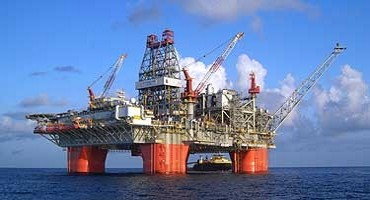
\includegraphics[width=5cm]{aux/examples/thunder-horse/thunder-horse-before}
\end{figure}
\end{frame}


\begin{frame}[hasprev=true, hasnext=true]
\frametitle{Thunder Horse}
\framesubtitle{Problem}

\begin{itemize}
	\item In mid July 2005, Hurricane Dennis swirled in the Gulf of Mexico.

	\item The platform was evacuated as a precaution.

	\item Upon return to the platform on July 12 2005, it was found
	precariously listing 20 to 30 degrees.
	\begin{itemize}
		\item The lower deck of the platform was at sea level.
	\end{itemize}
\end{itemize}

\begin{figure}
	\centering
	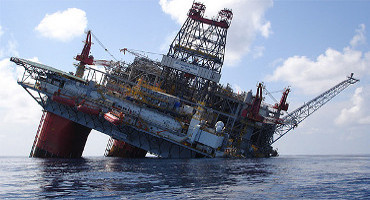
\includegraphics[width=5cm]{aux/examples/thunder-horse/thunder-horse-after}
\end{figure}
\end{frame}


\begin{frame}[hasprev=true, hasnext=false]
\frametitle{Thunder Horse}
\framesubtitle{Diagnostic}

\begin{itemize}
	\item Thunder Horse oilfield listing after an hurricane due to a ballast
	system error.
\end{itemize}
\end{frame}